\documentclass[a4paper, 12pt]{article}

%\usepackage{savetrees}
\usepackage{graphicx}
\usepackage{subfig}

%code for creating python code snippets
\usepackage{float}
\floatstyle{ruled}
\newfloat{python}{thp}{lop}
\floatname{python}{Listing}
%end code for creating python code snippets

\graphicspath{{./images/}}
\title {Student Robotics 2009\\ PWM Board Documentation}
\date{\today}
\setcounter{tocdepth}{1}


\begin{document}

\maketitle

\noindent This document describes the functions of the PWM/Servo Board. 

\begin{figure}
\centering
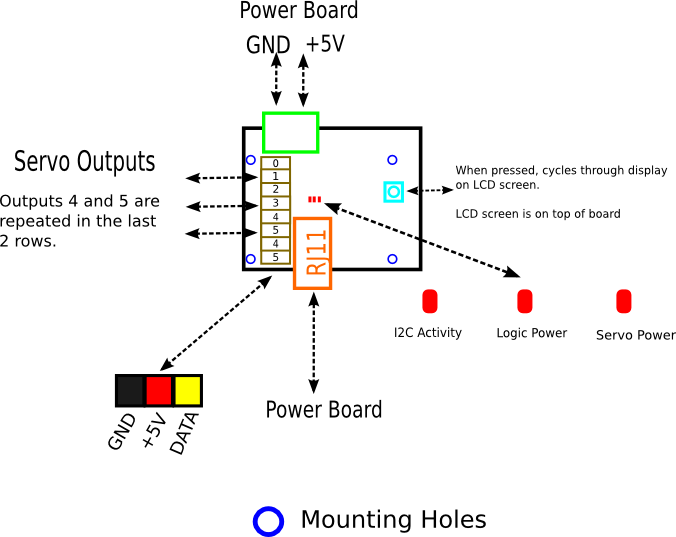
\includegraphics[scale=1, angle=90]{outline}
\caption{PWM Board 1:1 Scale Drawing}
\label{fig:outline}
\end{figure}


\section{Board Outline}
Figure \label{fig:outline} is a 1:1 scale drawing of the PWM board which can be printed out and used to aid drilling holes for mounting.
\label{sec:outline}

\section{Brief Description}

The PWM (Pulse Width Modulation) Board, often referred to as the Servo Board provides 6 independent servo channels for controlling a multitude of mechanical structures on your robot. 

In addition, this board also houses a 2x16 (2 rows of 16 characters) LCD display for providing live debug information.


For instructions on how to assemble the Servo board and Student Robotics kit, see \textit{Student Robotics Assembly Guide 2009}, available from the website.


\section{Connecting Servos}
\subsection{Types of Servo}
The PWM Board can control standard 5V PWM servos - such as those used in model planes/boats etc. 

\subsection{Connecting Servos}
Servos are connected to the PWM Board using the bank of vertical pin headers on the top side of the board as shown in figure \ref{fig:servo-header}. Each row of three pins corresponds to a single servo output. Be careful to ensure that the polarity is correct before connecting. 

\vspace{12pt}
\noindent {\bf Do not attach/detach servos whilst the PWM Board is on. This may damage the Board. }

\begin{figure}[h]
\centering
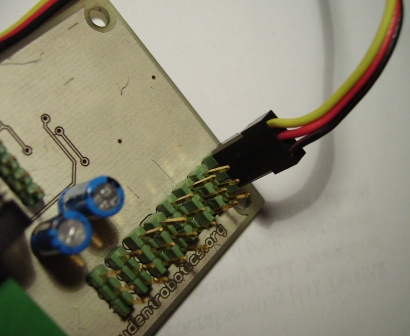
\includegraphics[scale=0.6, angle=0]{servo-header}
\caption{Connecting Servos to the PWM Board using the Pin Headers}
\label{fig:servo-header}
\end{figure}

\subsection{Duplicate Outputs}
Although there are eight rows of pin headers on the PWM Board, the last two headers are duplicates of servos 4 \& 5 - see figure \ref{fig:outline}.  

\section{LCD}
During testing you may want to write text to the LCD from within your python robot code. This could help to determine how far into your program you are. Other possibilities include:

\begin{itemize}
\item Write a message to LCD when camera detects a blob
\item Writing error messages to the LCD
\item Show alert when sensors detect wall/ball
\item View JointIO input/output status 
\end{itemize}

The push switch on the PWM Board allows you to cycle through which message or page of text is displayed. 
\vspace{12pt}

For information on how to write text to the LCD, please refer to the Programming Reference, available on the website.

\section{Troubleshooting}
\subsection{Servos Do Not Move}
Have you ensured the polarity of the servo conenctor matches with figure \ref{fig:outline}? Is the 5V rail connected to the Power Board? Is your servo connected to the correct pin header?

\end {document}
